\documentclass[a4paper]{scrartcl}

%% Language and font encodings
\usepackage[english]{babel}
\usepackage[utf8x]{inputenc}

%% Sets page size and margins
\usepackage[a4paper,top=2cm,bottom=3cm,left=1.9cm,right=1.7cm]{geometry}

%% Useful packages
\usepackage{graphicx}
\usepackage[colorlinks=true, allcolors=blue]{hyperref}
\usepackage[skip=3pt, format=plain]{caption}
\renewcommand\thesection{\Alph{section}}
%\usepackage{multicol}

\title{Computational Motor Control - Lab 5}
\subtitle{Modelling the salamander CPG with phase oscillators}
\author{Florian Kaufmann \and Octave Martin \and Matthias Tsai}

\begin{document}

{\twocolumn

\setlength{\columnsep}{0.5cm}
\maketitle

\section{Running the CPG model}

The salamander CPG model was first tested by simulating the system for 20 seconds while applying a constant drive of 4.5 (see figure \ref{fig:7a-swim}). One can observe that after a short adaptation period, the various frequencies of the axial oscillators quickly join to converge at a frequency around 1.2 Hz resulting in a synchronized linear phase gradient from the upper axial oscillators downwards as observed in real swimming salamander. The phase difference between the first and the last oscillator is also approximately $2\pi$, which corresponds to the natural swimming behaviour of the salamander. Finally, one should also note that as expected the limbs are completely inactive during the simulation except maybe for the very beginning, during which the system needs to stabilize its random initial state.

Next the simulation of the salamander CPG was repeated, but applying a drive of only 2.5 this time (see figure \ref{fig:7a-walk}). This resulted in a low frequency anti-phase oscillation of the two limb oscillators. Through the coupling of the limb oscillators to the axial oscillators, the latter displayed two different type of behaviour depending if they were located in the upper or lower half of the body although all of them synchronized to the frequency of the limb oscillators around 0.5 Hz. The upper axial oscillators are in anti-phase to the upper limb oscillator and the lower axial oscillators are in anti-phase with the lower limb oscillator. Again this stable state is only achieved after a short and noisy adaptation period, but the result is very close to what is experimentally observed in a salamander. One can observe how the activity of the limbs regulates the oscillation frequency of the body trunk by letting it oscillate at high frequency during swimming, but taking over the control of the trunk frequency when walking.

\begin{figure}[!h]	
	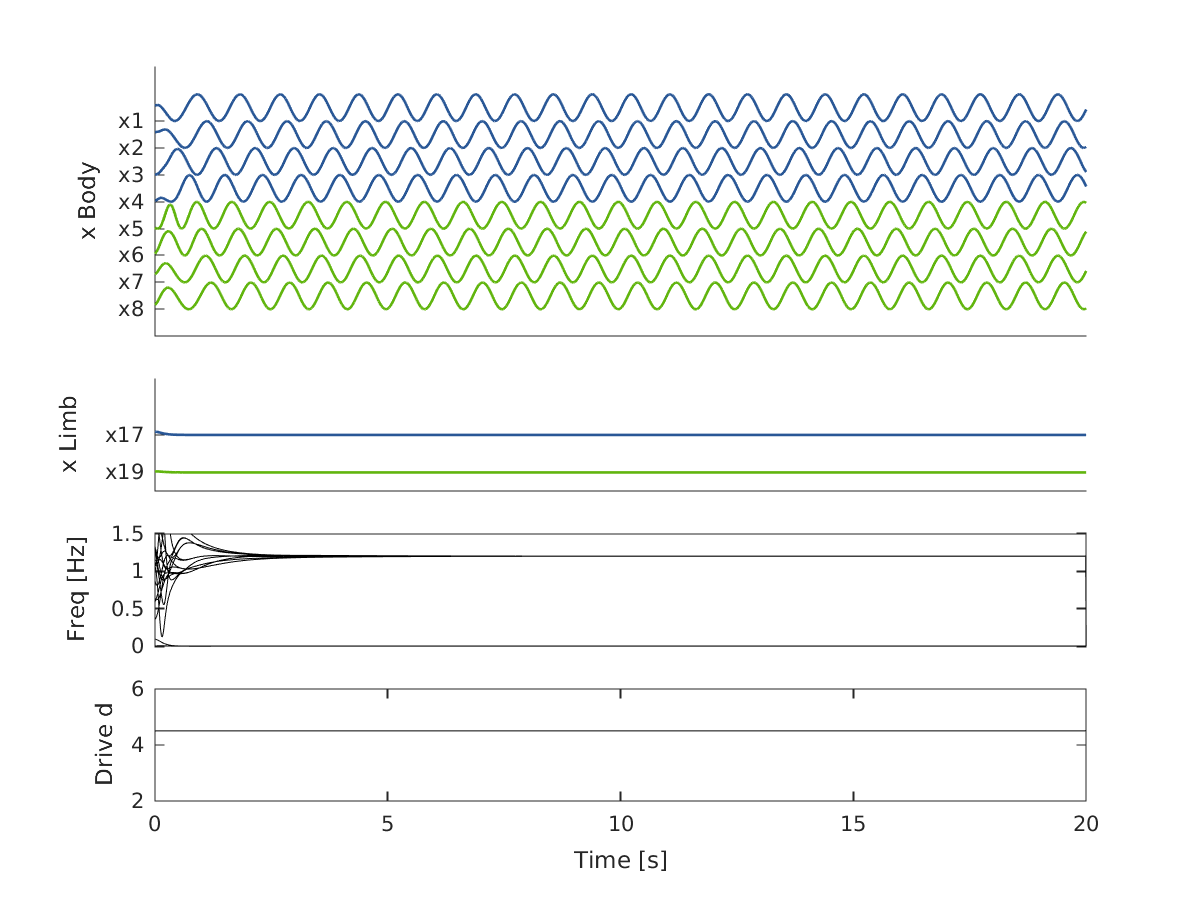
\includegraphics[width=0.5\textwidth]{fig/figure7a-swim.png}
	\caption{Simulation of the salamander CPG model for a duration of 20 seconds while applying a constant drive of 4.5 and resulting in a steady swimming behaviour.}
	\label{fig:7a-swim}
\end{figure}

\begin{figure}[!h]
	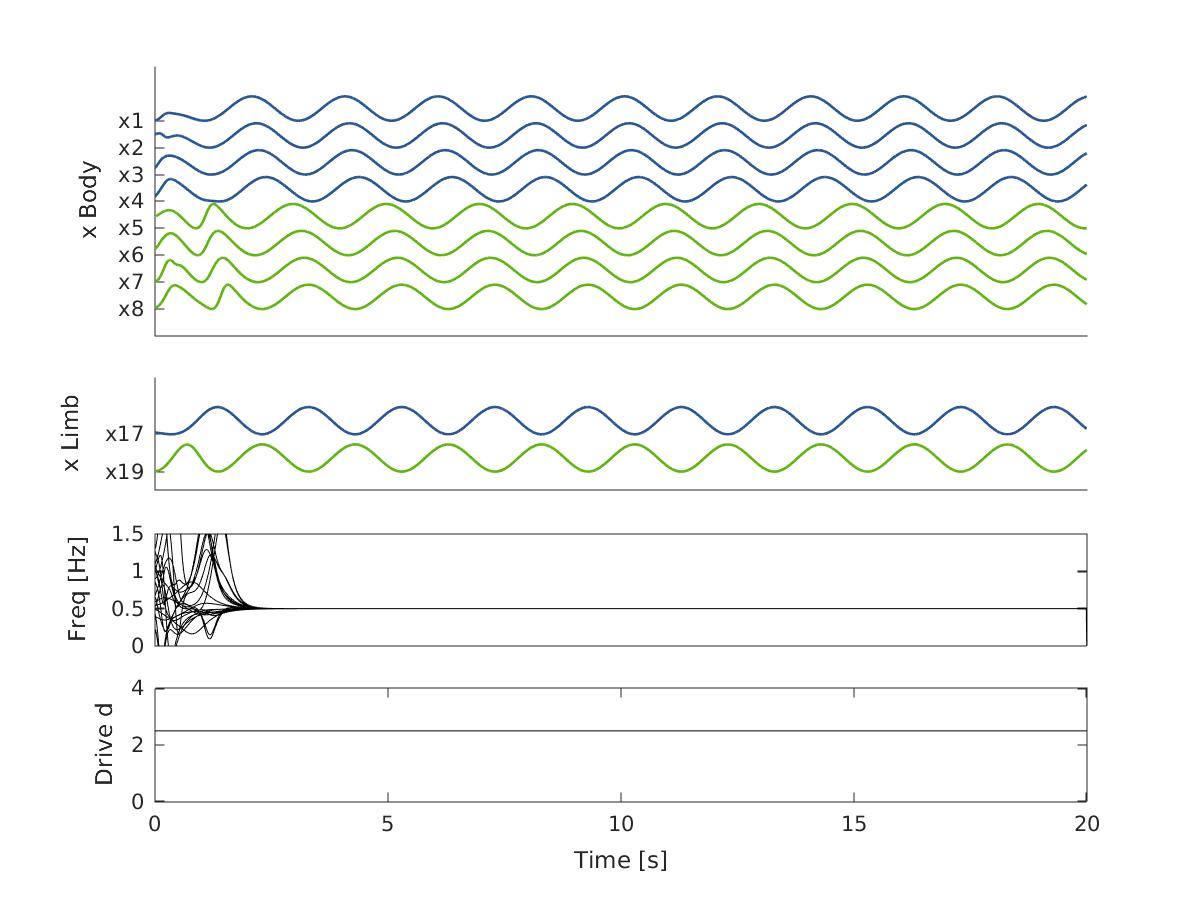
\includegraphics[width=0.5\textwidth]{fig/figure7a-walk.png}
	\caption{Simulation of the salamander CPG model for a duration of 20 seconds while applying a constant drive of 2.5 and resulting in a steady walking behaviour.}
	\label{fig:7a-walk}
\end{figure}

\begin{figure}[!h]
	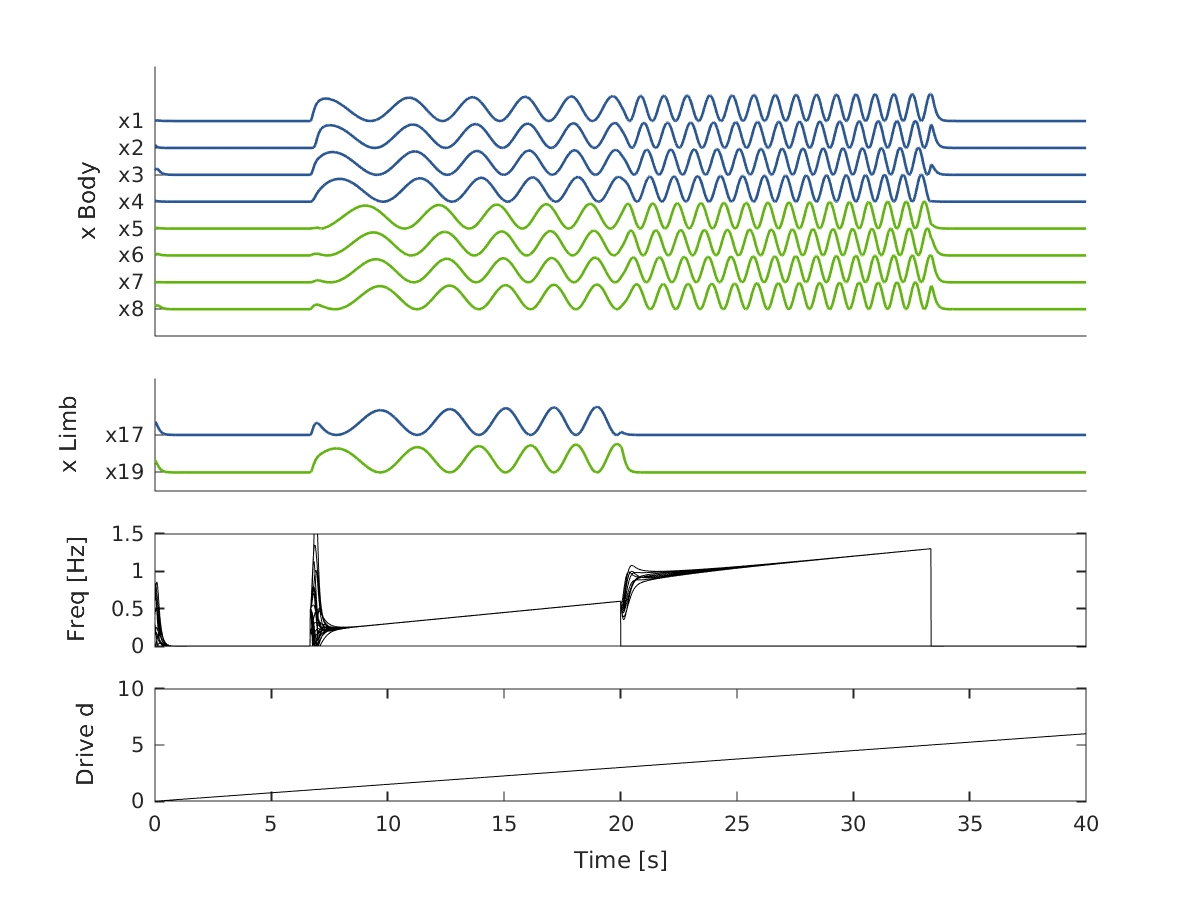
\includegraphics[width=0.5\textwidth]{fig/figure7a-drivegradient.png}
	\caption{Simulation of the salamander CPG model for a duration of 40 seconds while applying a linearly increasing drive from 0 to 6 and resulting in a transition from rest to walking to swimming and back to rest.}
	\label{fig:7a-transition}
\end{figure}

To analyse the transition from a walking to a swimming behaviour another simulation was run during which the model was subjected to a linearly increasing drive from 0 to 6 (see figure \ref{fig:7a-transition}). Up to around second 7 into the simulation, the CPG model stabilizes into resting mode, during which all limb and axial oscillators are inactive. Around 7 seconds into the simulation, the drive reaches a value of 1, which is the threshold value at which all oscillators have a non-zero intrinsic frequency (see figure \ref{fig:7a-saturation}), thus driving the system to oscillate. The system then starts off in a chaotic manner before stabilizing in a walking behaviour as previously described in figure \ref{fig:7a-walk}, but with linearly increasing frequency. Since the intrinsic frequencies of the oscillators and more importantly the limb oscillators has a linear dependence on the drive for values between 1 and 3, it is not surprising that the walking frequency increases with the linearly increasing drive. Once the drive reaches a value of 3 around 20 seconds into the simulation the walking behaviours suddenly stops before rapidly being replaced by a swimming behaviour. As seen before with the walking phase and because the intrinsic frequency of the axial oscillators is also linearly dependent on the drive, the swimming frequency also increases linearly for a while, although one should note that the axial oscillators had experienced a sudden jump in frequency once the limb oscillators were inactivated around the 20th second of simulation. This jump is due to the constant difference in intrinsic frequencies between limb and axial oscillators in the walking range of the drive between 1 and 3. In this range the axial oscillators have an intrinsic frequency about a quarter Hertz above the intrinsic frequency of the limb oscillators at any time, but are held down the limb frequency through a coupling strength as observed in figure \ref{fig:7a-walk}. Finally, around 33 seconds into the simulation, the drive reaches a value of 5, which is the threshold value above which the intrinsic frequency of the axial oscillators also goes to zero (see figure \ref{fig:7a-saturation}), which explains why the CPG model returns to a resting state at which all oscillators remain quite.

\begin{figure}[!h]
	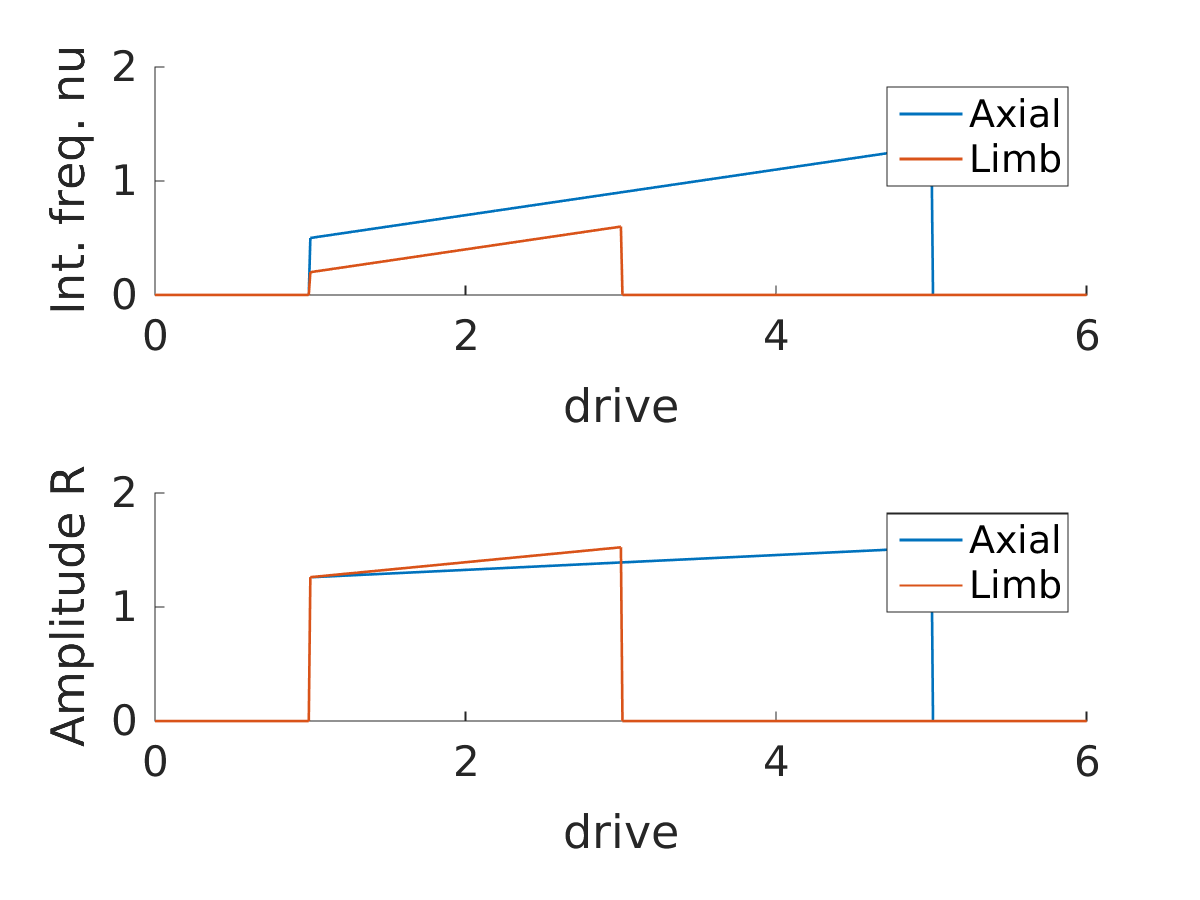
\includegraphics[width=0.5\textwidth]{fig/figure7a-frequency-drive-dependence.png}
	\caption{Plot of the frequency dependence of the intrinsic frequencies and amplitudes of axial and limb oscillators.}
	\label{fig:7a-saturation}
\end{figure}


\section{Handling of perturbations}
Natural systems, such as the salamander are constantly subjected to noise, both internal and external. The CPG model's robustness when faced to noise was therefore tested. First, the system was simulated when subjected to a noisy drive with linearly increasing noise variance in time (see figure \ref{fig:7b-drive}). This was performed using both an average drive of 2 and of 4 to compare the stability of the walking and the swimming behaviour to noise and both displayed a qualitatively similar dynamic. The oscillators maintained a clean oscillation up to a variance of 0.5, where they started to develop a visible high frequency noise. However the swimming and walking frequencies remain relatively intact up to a noise variance around 1, at which point the low frequency oscillations are more notably disturbed and start to slightly slow down. This behaviour intensifies until the main walking and swimming oscillation start to completely break down when subjected to noise of variance approximately 1.5 and the main frequencies have decreased by half. From there on the oscillators become more and more random, but one should note that they maintain a good correlation. Most noticeably for the swimming case, the phase gradient the axial oscillators is visible for the low frequency component at least up to a noise variance of 4 and despite the constant decrease in frequency of this synchronized oscillations. Furthermore the phase difference between the uppermost and lowest axial oscillator also seems to stay around $2\pi$ no matter what. For the walking case, it 
seems that through the loss of the limb oscillation the walking structure of 

\begin{figure}[!h]
	%\textbf{A}
    	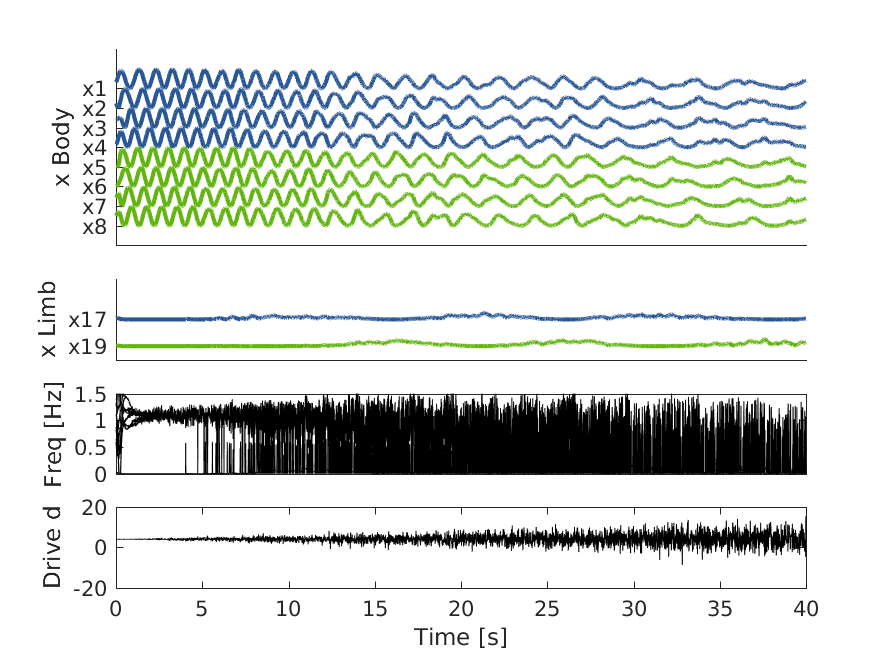
\includegraphics[width=0.5\textwidth]{fig/figure7b_drive-increasing-gaussian-swim.png}
    %\textbf{B}
	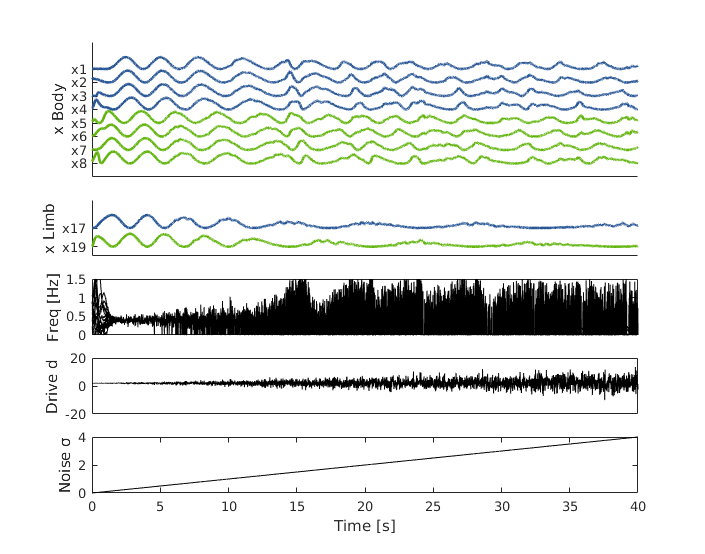
\includegraphics[width=0.5\textwidth]{fig/figure7b_drive-increasing-gaussian-walk.png}
	\caption{Simulations of the salamander CPG model with drive of constant mean, but linearly increasing noise variance from 0 to 4. Upper: Simulation in swimming mode with drive mean of 4. Lower: Simulation in walking mode with drive mean of 2.}
	\label{fig:7b-drive}
\end{figure}

{\setlength{\parindent}{0 cm}
the axial oscillator phases is lost and switches to a linear phase gradient similar to the noisy swimming.This supports the point made above, stating that the axial walking oscillations observed for low drive are induced by the limb oscillator, which restrains the more natural swimming oscillation of the axial oscillator. In case of strong noise acting on the limbs, this induced walking behaviour of the axial oscillators is lost, leading the system to recover its more intrinsic linear phase gradient.
}

Applying noise to the drive simulates intrinsic perturbations of the salamander like the noisy na-

\begin{figure}[!h]
	%\textbf{A}
    	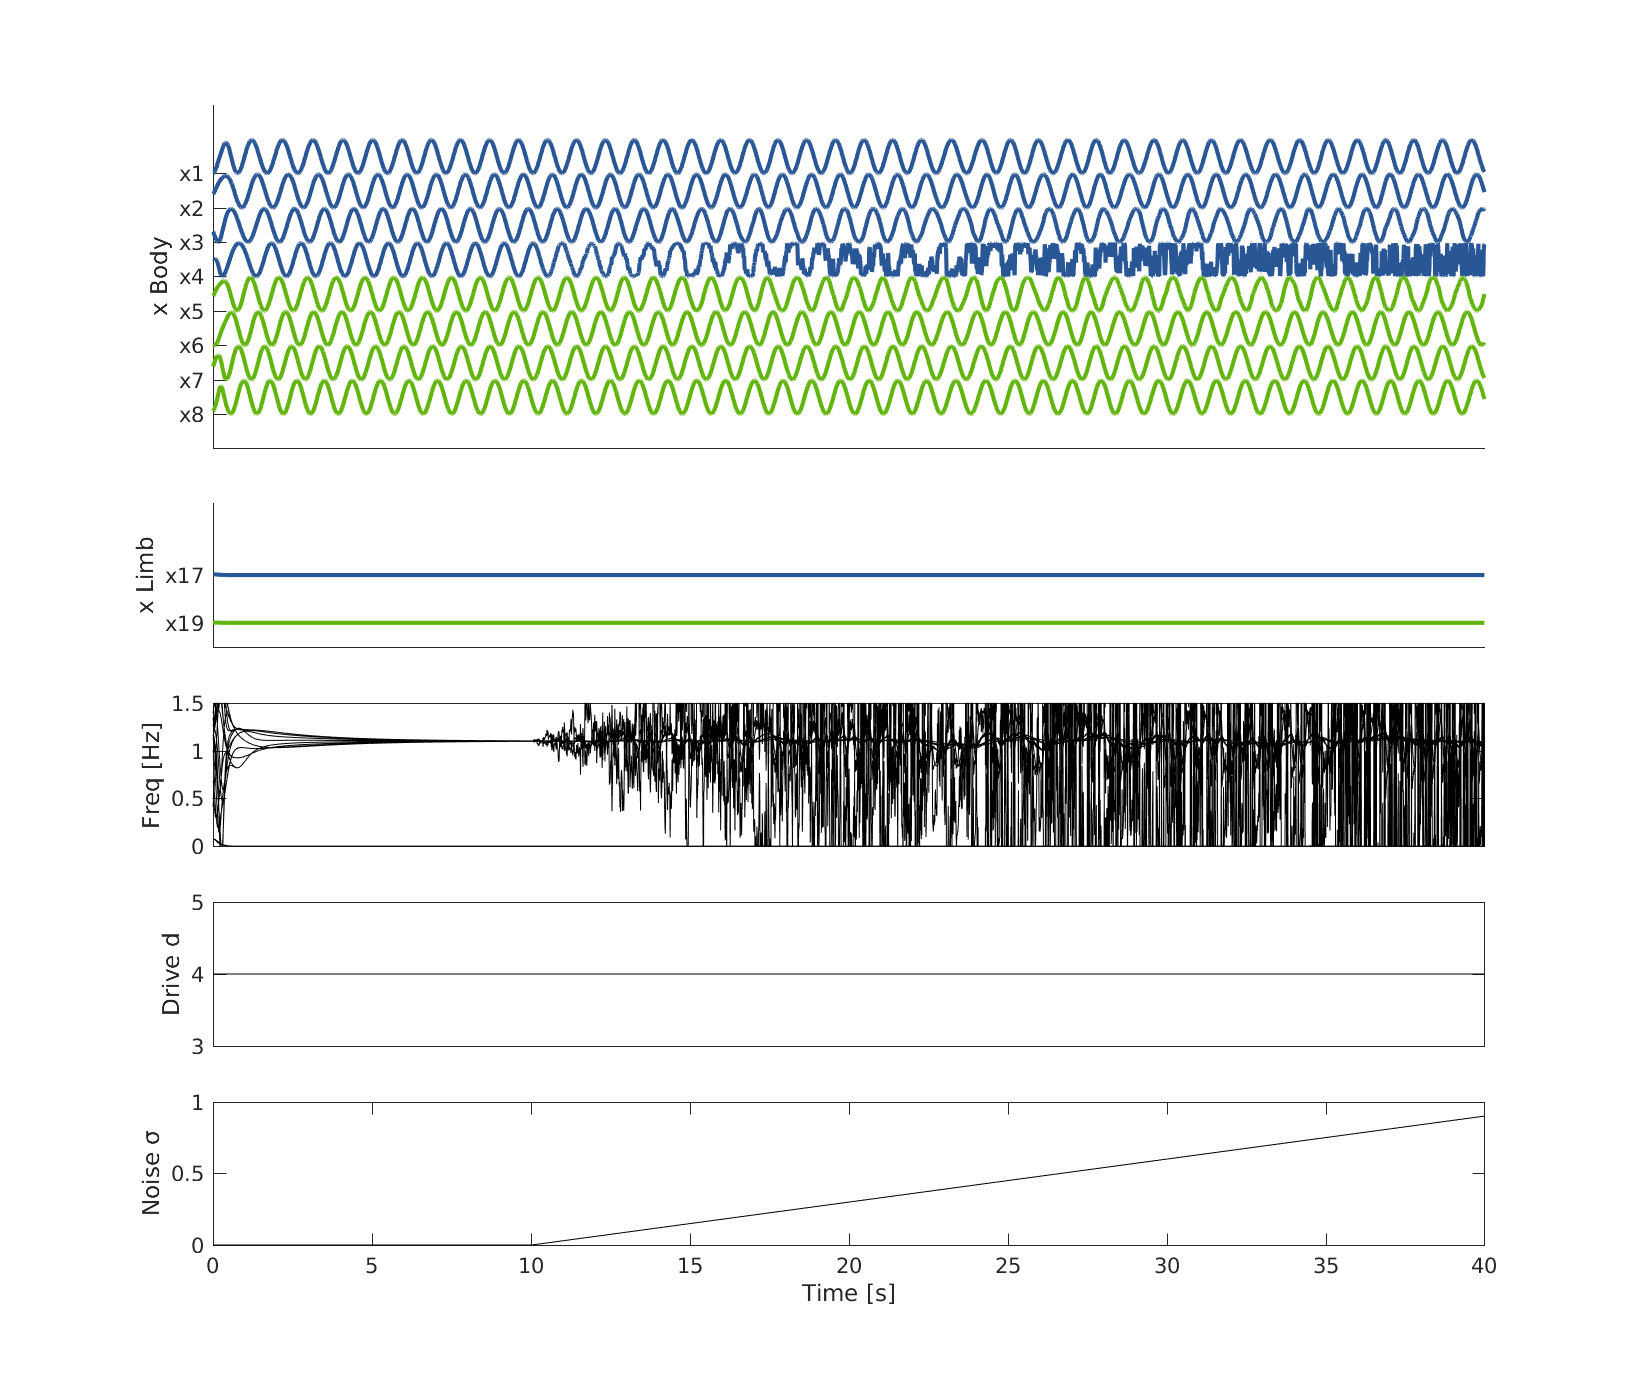
\includegraphics[width=0.5\textwidth]{fig/figure7b_axialphase-swim.png}
    %\textbf{B}
	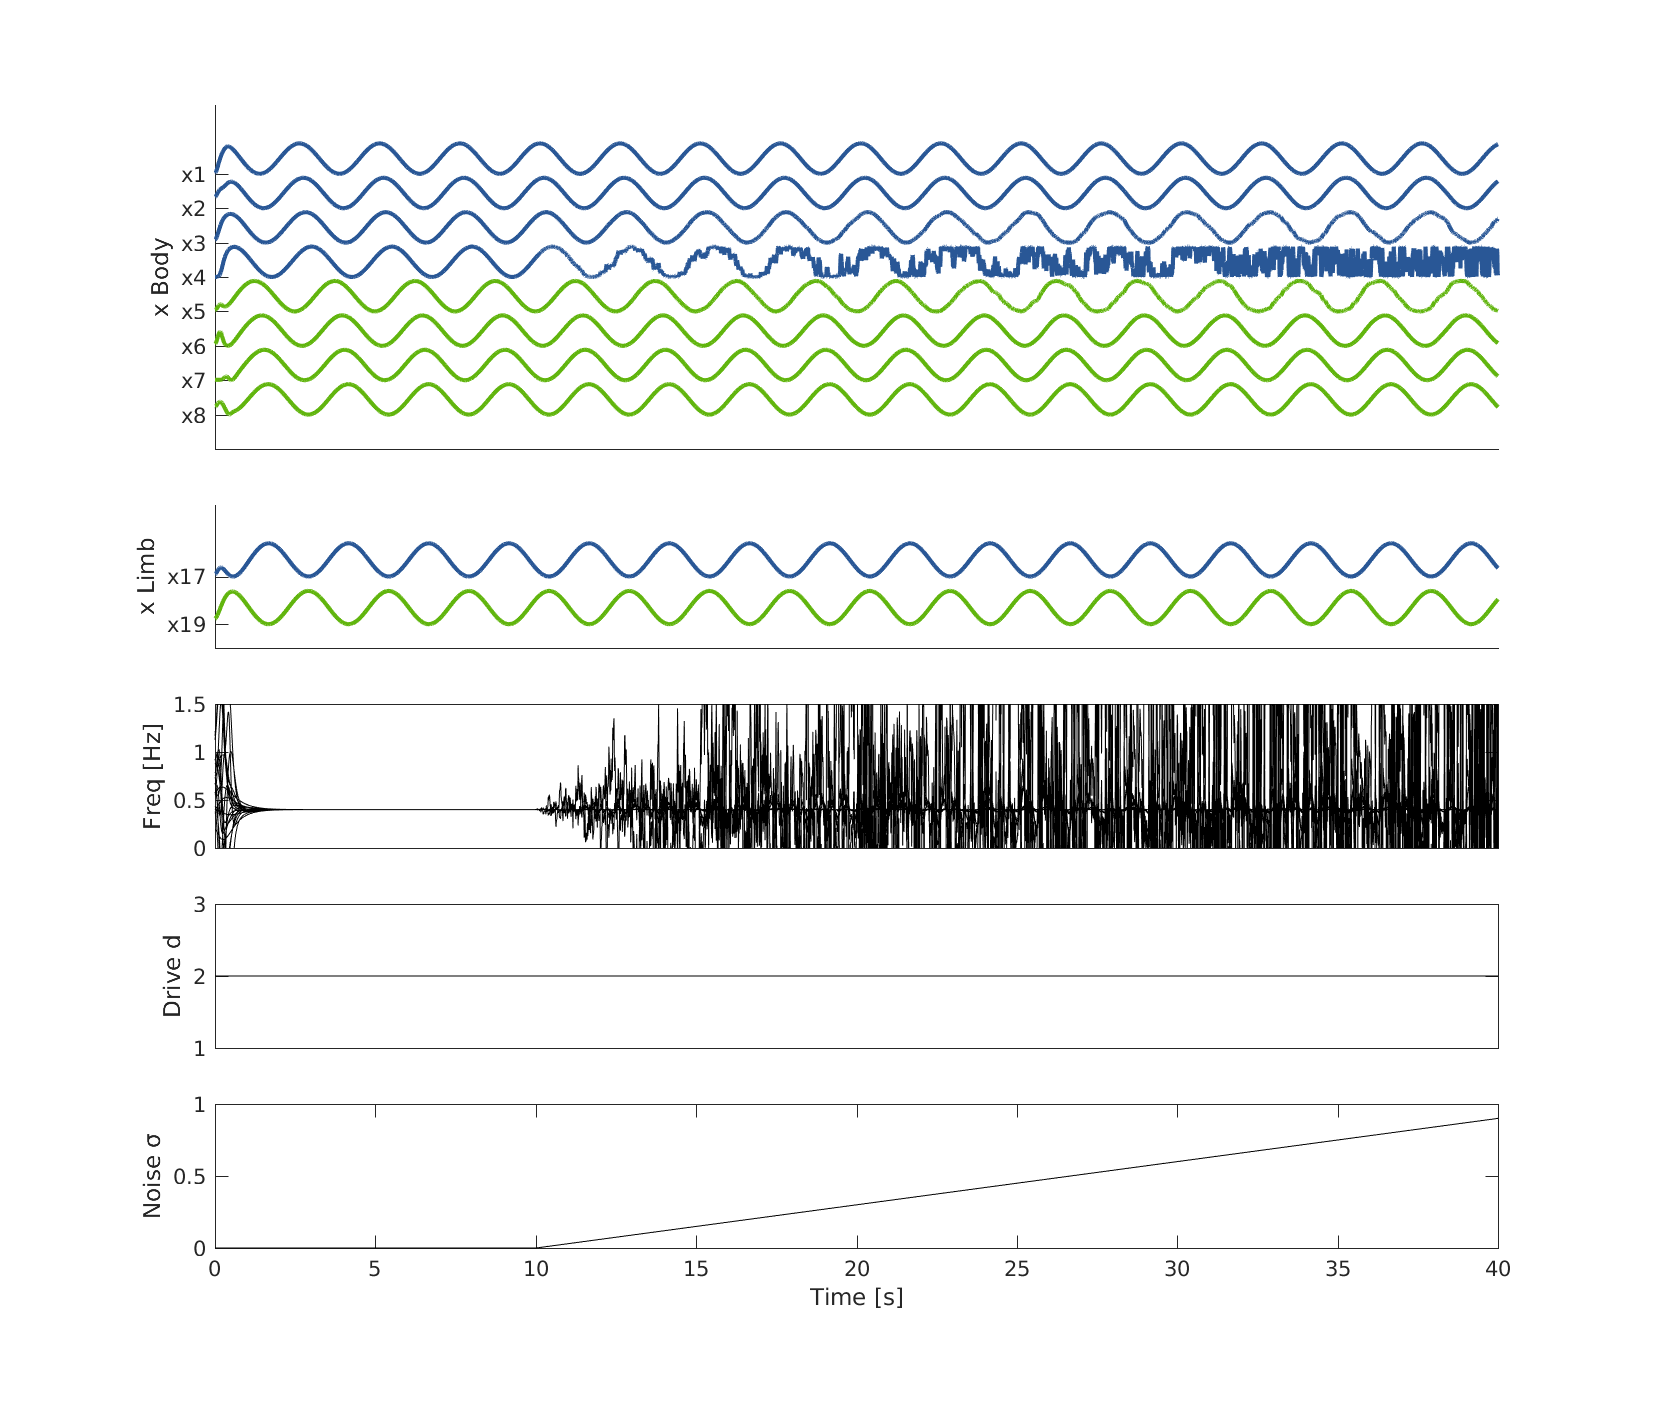
\includegraphics[width=0.5\textwidth]{fig/figure7b_axialphase-walk.png}
	\caption{Simulations of the salamander CPG model applying a perturbation on the fourth axial oscillator starting at 10 seconds into the simulation with a linearly increasing perturbation variance from 0 to 0.9. Upper: Simulation in swimming mode with constant drive of 4. Lower: Simulation in walking mode with constant drive of 2.}
	\label{fig:7b-allphase}
\end{figure}

{\setlength{\parindent}{0 cm}
ture of its brain. In the next step, mechanical perturbations were simulated by applying increasing noise to the phases of the oscillators. When the noise was applied to a single axial oscillator (see figure \ref{fig:7b-allphase}) either during walking or swimming behaviour. One can observe that in both cases, although the perturbed oscillator becomes increasingly noisy and random, the other oscillators are all minimally perturbed and maintain their overall phase structure.
}

The simulation in walking mode was repeated, but applying the perturbation on a limb oscillator this time (see figure \ref{fig:7b-limbphase}). In this case the perturbation on the upper limb oscillator had a distinct effect on all the upper axial oscillators. However, one should also note that even when the perturbation had grown such that the limb oscillator had become almost complete noise, the upper axial oscillators maintained a dynamic that allowed to recognize a walking behaviour. This is most probably due to the coupling between the lower and the upper axial oscillators. This can also be seen in the fact that the upper oscillators that are located more centrally and thus closer to the lower oscillators and are subjected to a stronger coupling to these lower oscillators, are less sensitive to the perturbation transmitted by the upper limb oscillator and maintain a cleaner walking oscillation than the uppermost oscillators.

\begin{figure}[h]
	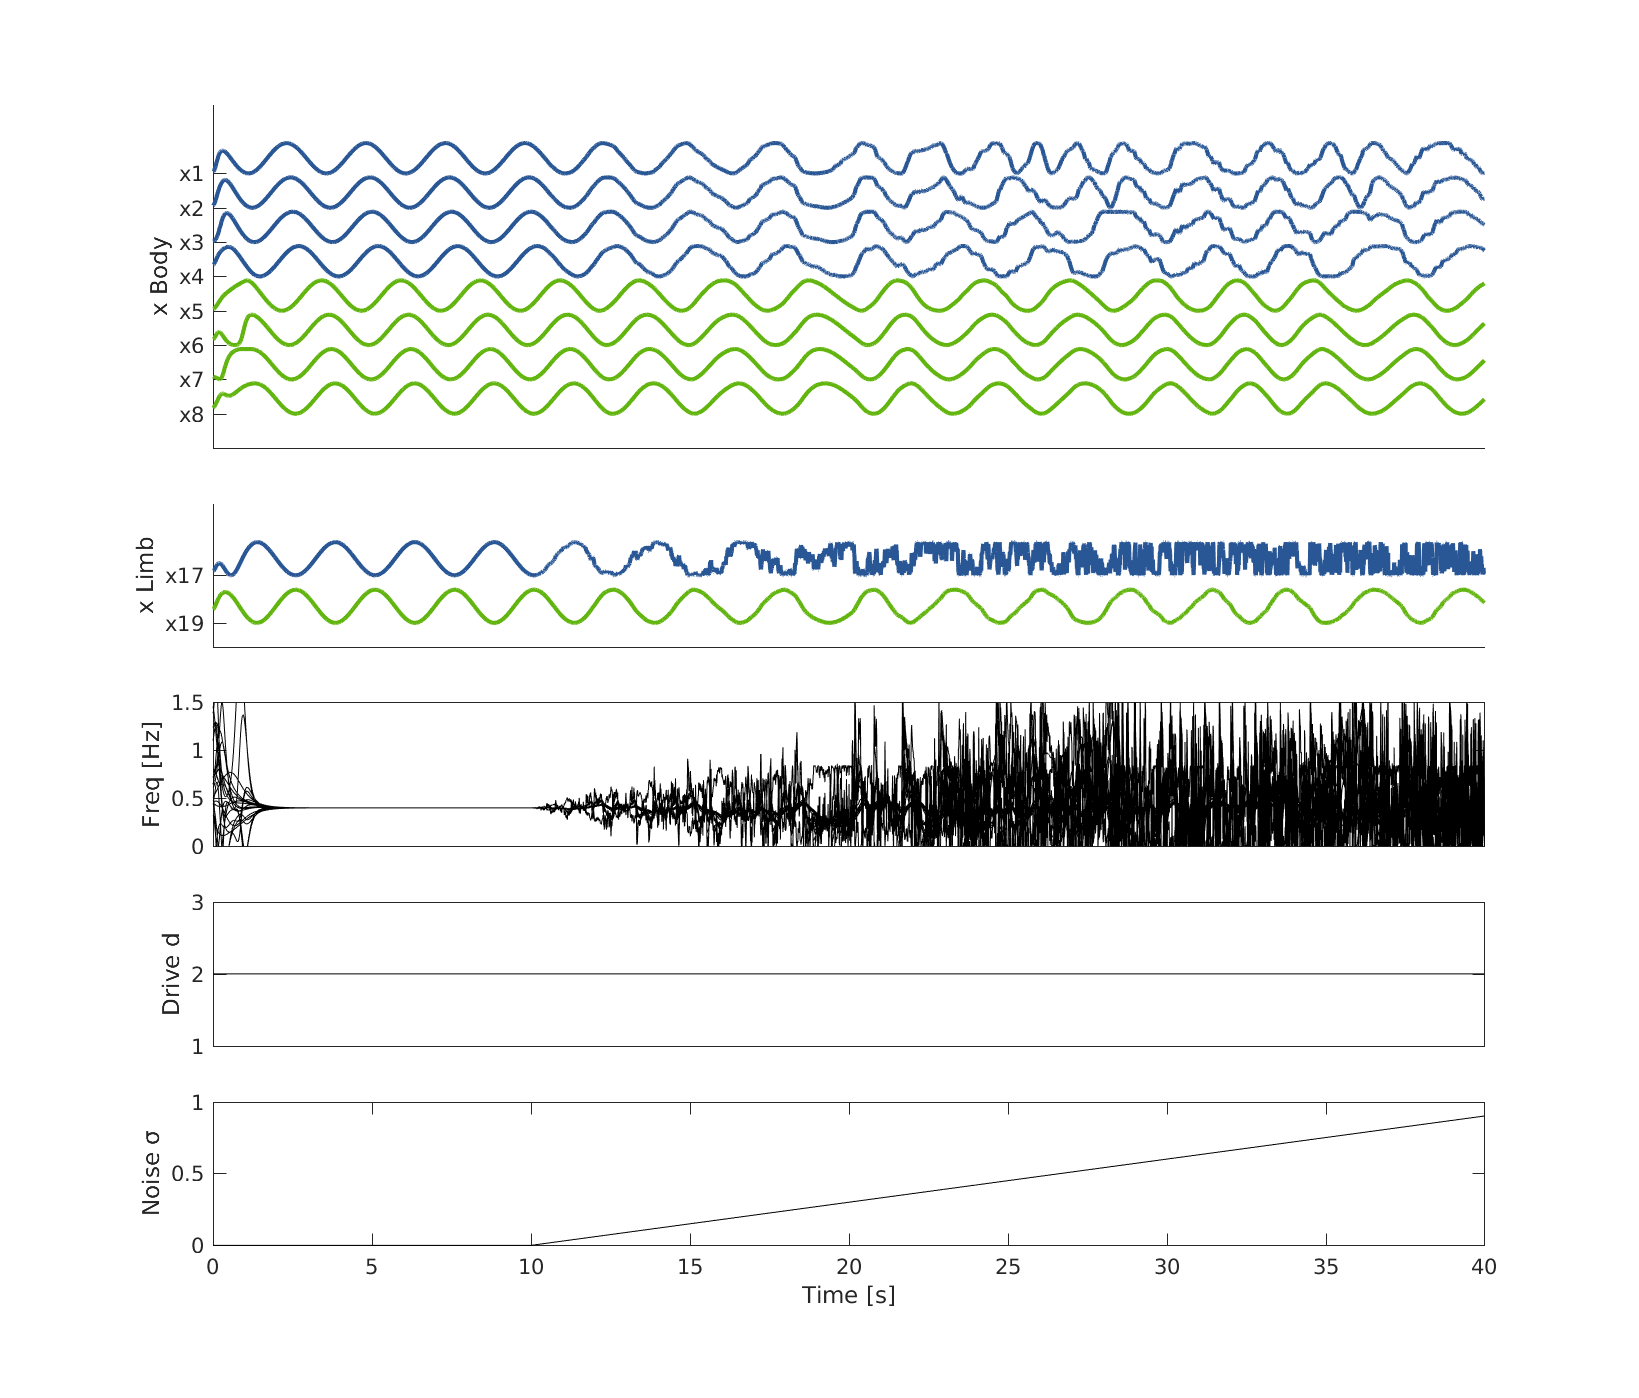
\includegraphics[width=0.5\textwidth]{fig/figure7b_limbphase.png}
	\caption{Simulation of the salamander CPG model applying a perturbation on an upper limb oscillator starting at 10 seconds into the simulation with a linearly increasing perturbation variance from 0 to 0.9.}
	\label{fig:7b-limbphase}
\end{figure}

Finally, perturbations were applied to all oscillators both during swimming and walking mode. The perturbation of the drive simulated intrinsic noise, like intrinsic noise in the brainstem, while the single oscillator perturbation simulated a more mechanistic noise on a single body part, like a torn muscle or a completely external mechanical input. This last simulation models a broader kind of environmental mechanic noise, like turbulent water. The outcome of this simulation (see figure \ref{fig:7b-allphase}) shows that the CPG model can sustain perturbations and maintain a clean swimming behaviour up to a noise

\begin{figure}[!h]
	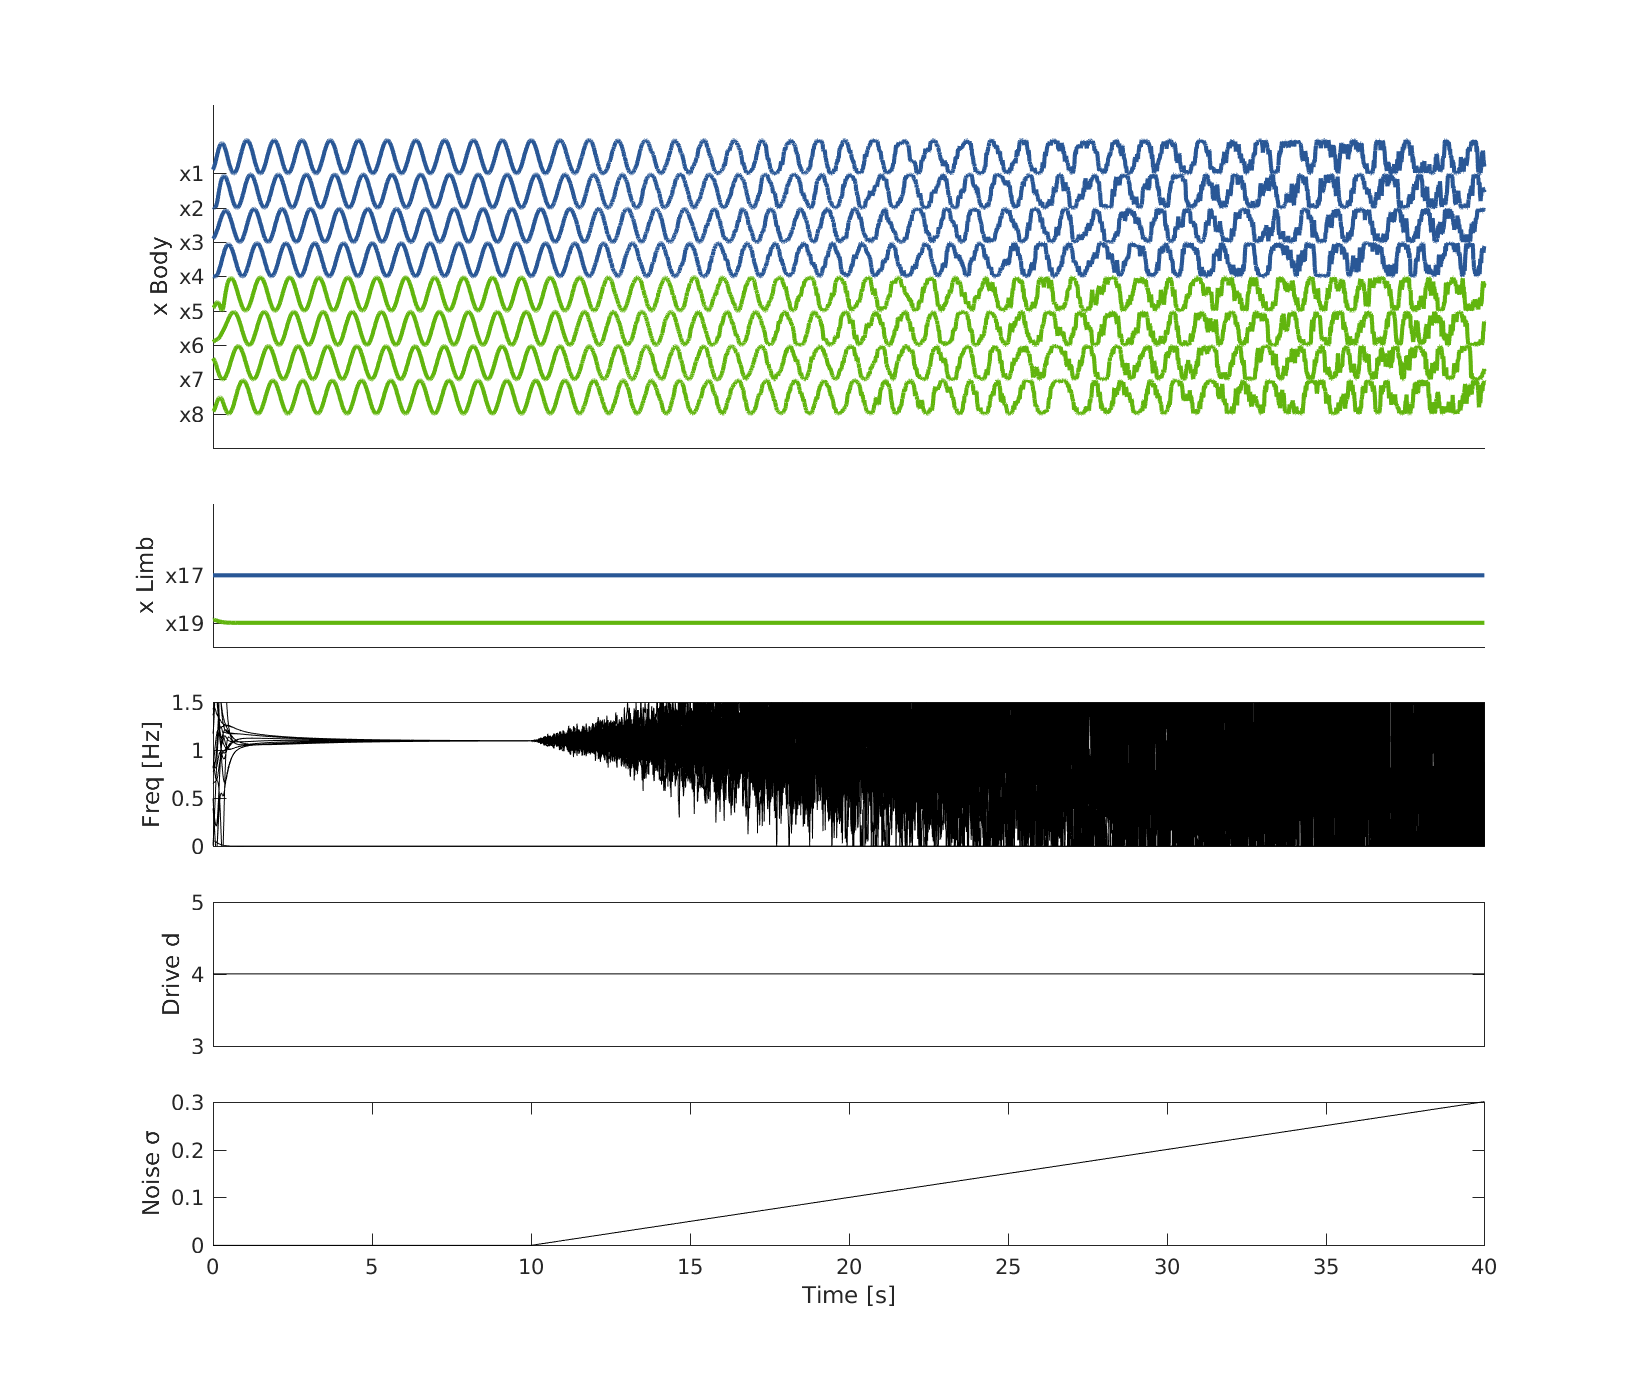
\includegraphics[width=0.5\textwidth]{fig/figure7b_allphase-swim.png}
	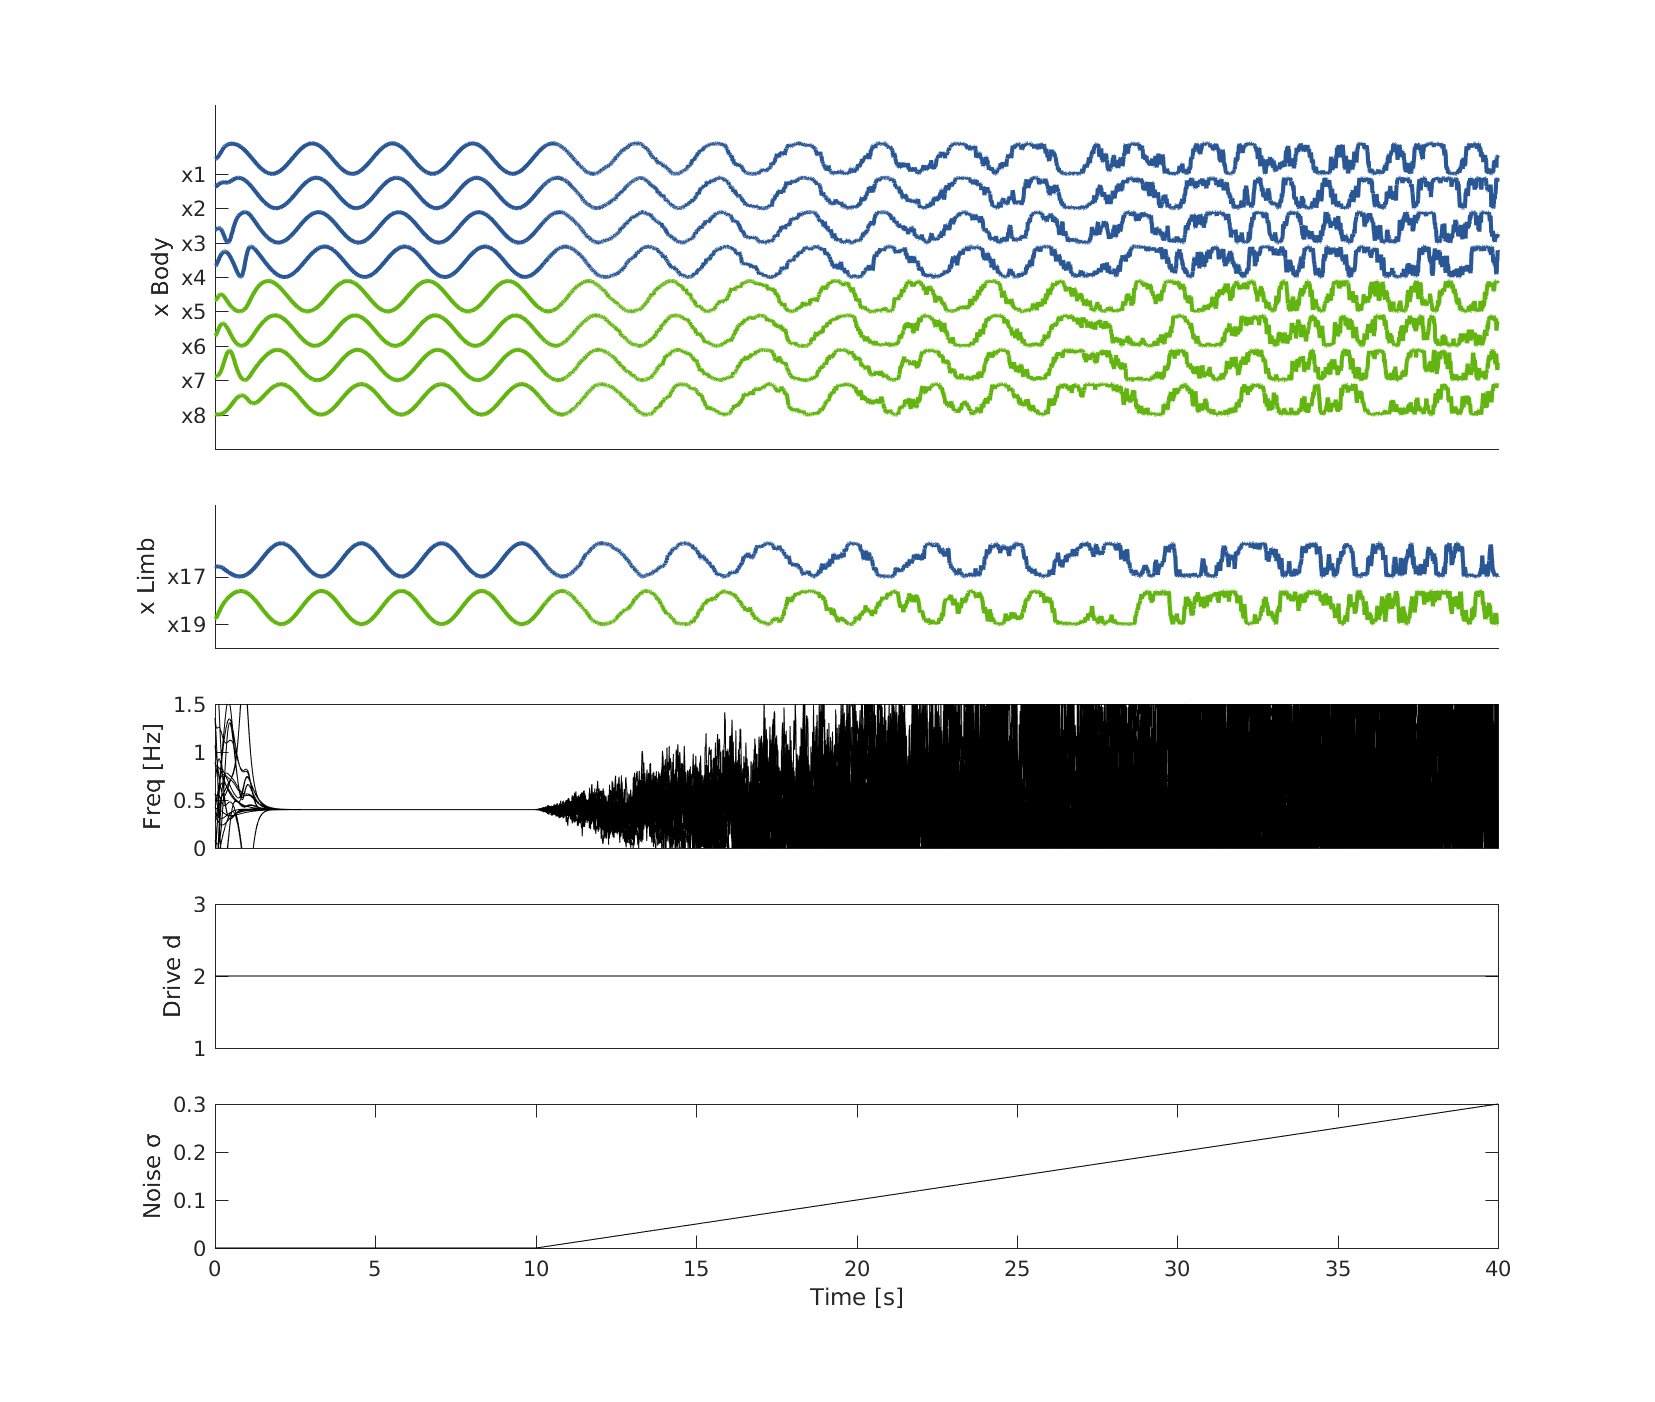
\includegraphics[width=0.5\textwidth]{fig/figure7b_allphase-walk.png}
	\caption{Simulations of the salamander CPG model applying a perturbation on all oscillators starting at 10 seconds into the simulation with a linearly increasing perturbation variance from 0 to 0.9. Upper: In swimming mode with constant drive of 4. Lower: In walking mode with constant drive of 2.}
	\label{fig:7b-allphase}
\end{figure}

{\setlength{\parindent}{0 cm}
variance around 0.2 and a clean walking behaviour up to a noise variance around 0.15. One can also observe that the perturbation of the oscillators induces an increasingly strong jittering effect on the resulting dynamics that ends up in complete noise, while the drive perturbation induced a weakened and less smooth oscillation that however maintained a low frequency oscillators behaviour surprisingly long. This is a good indication that the CPG model is more robust to drive perturbation than direct mechanical perturbations, which shows that the spinal CPGs are good at compensating for a noisy input from the brain. One should note that the relatively poor robustness of the system to mechanical perturbations could be improved by adding sensory inputs to the oscillators that would compensate for external noise.
}

\section{Playing with model parameters}

In this section, the influence of the various parameters was studied and various simulations were run with different values for selected parameters. The First parameter investigated was the axial coupling. 

\begin{figure}[!h]
	\hspace*{-1 cm}
	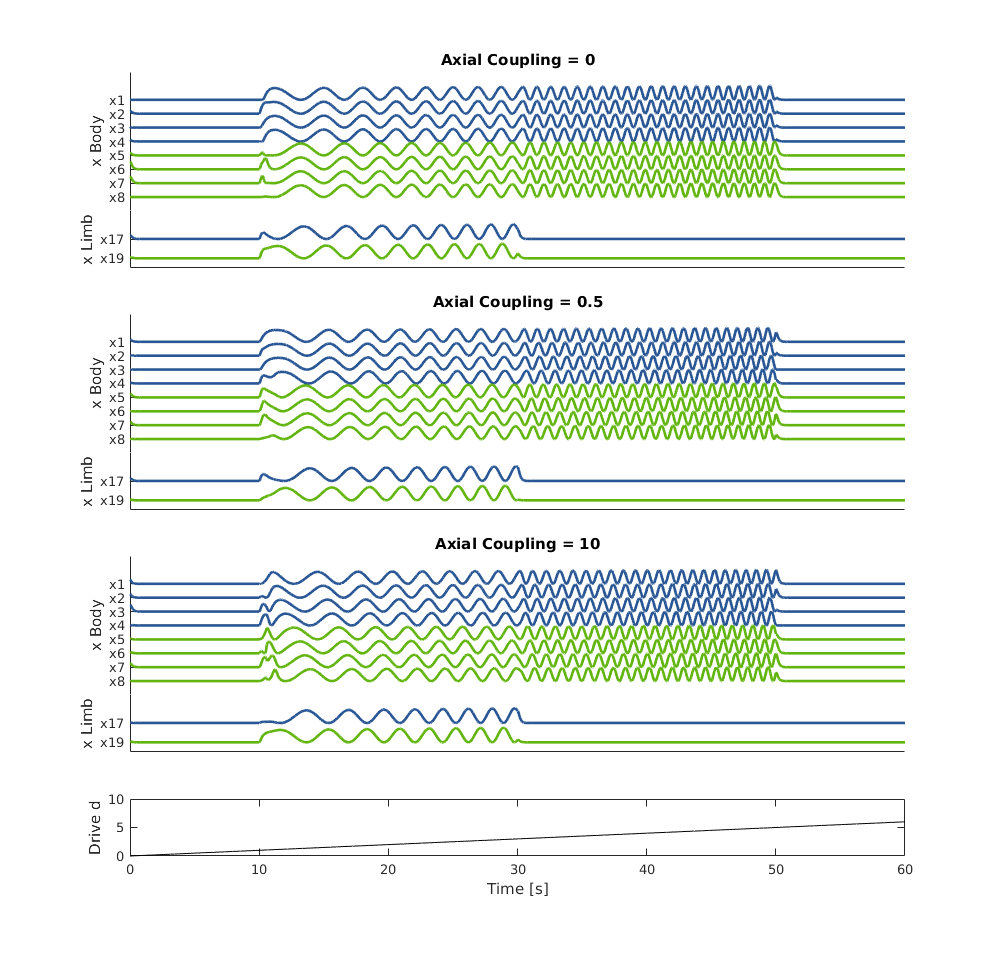
\includegraphics[width=0.6\textwidth]{fig/figure7c_axial-coupling.png}
	\caption{Simulations of the salamander CPG model applying a linearly increasing drive with three different values for axial coupling values (0, 0.5 and 10).}
	\label{fig:7c-axialcoupling}
\end{figure}

{\setlength{\parindent}{0 cm}
In a first round of simulation the upward and downward axial coupling strengths were both set at either 0, 1 or 10 (see figure \ref{fig:7c-axialcoupling}). This showed how a too weak axial coupling (for a value = 0) could lead to a good walking behaviour, but a loss in swimming dynamic. On the other side, a too strong axial coupling (for a value = 10) could lead to a good swimming behaviour, but a loss in walking dynamic. This shows that a good value (e.g. around 0.5) can allowed a sufficiently strong axial coupling, leading to a phase gradient for the swimming behaviour, but was still not too strong, such that it allowed the coupling from the limbs to take over the control of the axial dynamics during walking.
}

To also visualize the individual role of the coupling strength of the limbs on the axial oscillators a similar protocol was applied using a constant drive of 2 to produce walking (see figure \ref{fig:7c-limbaxialcoupling}). This shows how important this coupling is in order for the limbs to overrun the default swimming behaviour of the axial oscillators during walking. Indeed for a value of zero the trunk and tail of the animal produce a slow swim-like motion and for a low value

\begin{figure}[!h]
	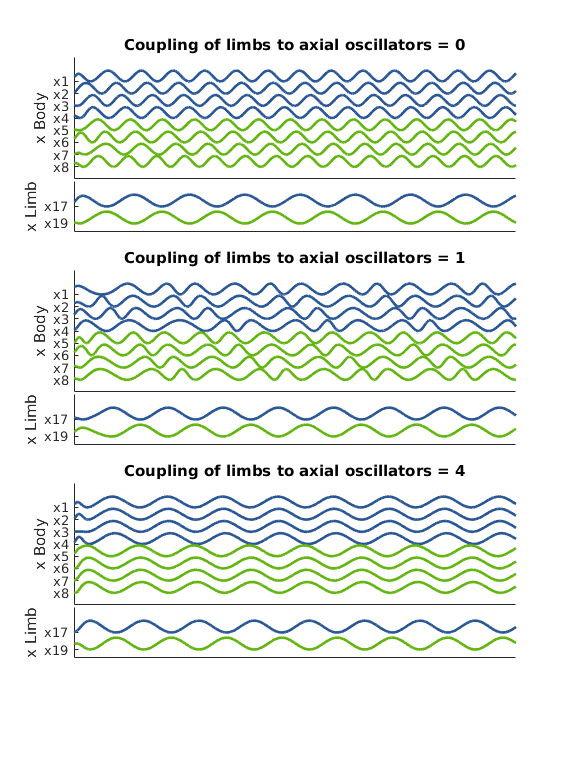
\includegraphics[width=0.5\textwidth]{fig/figure7c_limbaxial-coupling.png}
	\vspace*{-1.5 cm}
	\caption{Simulations of the salamander CPG model applying a constant drive of 2 to achieve walking with three different values for the coupling strength of the limbs on the axial oscillators (0, 1 and 4).}
	\label{fig:7c-limbaxialcoupling}
\end{figure}

\begin{figure}[!h]
	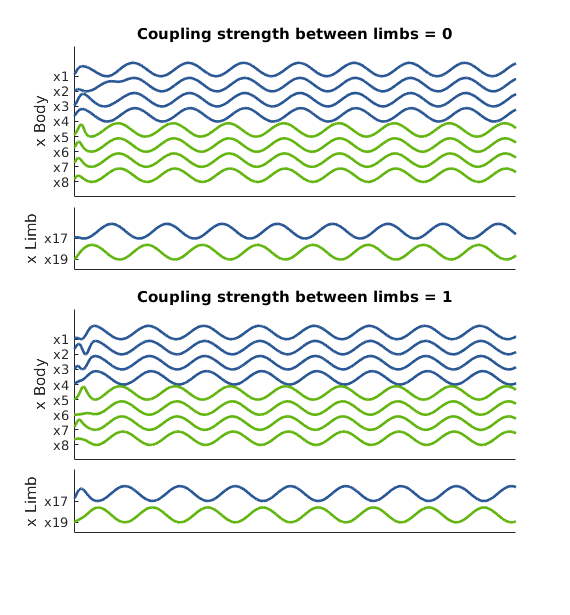
\includegraphics[width=0.5\textwidth]{fig/figure7c_limb-coupling.png}
	\vspace*{-1.5 cm}
	\caption{Simulations of the salamander CPG model applying a constant drive of 2 to achieve walking with two different values for the coupling strength between the limb oscillators (0 or 1).}
	\label{fig:7c-limbcoupling}
\end{figure}

} %twoclumn


\begin{figure*}[!b]
	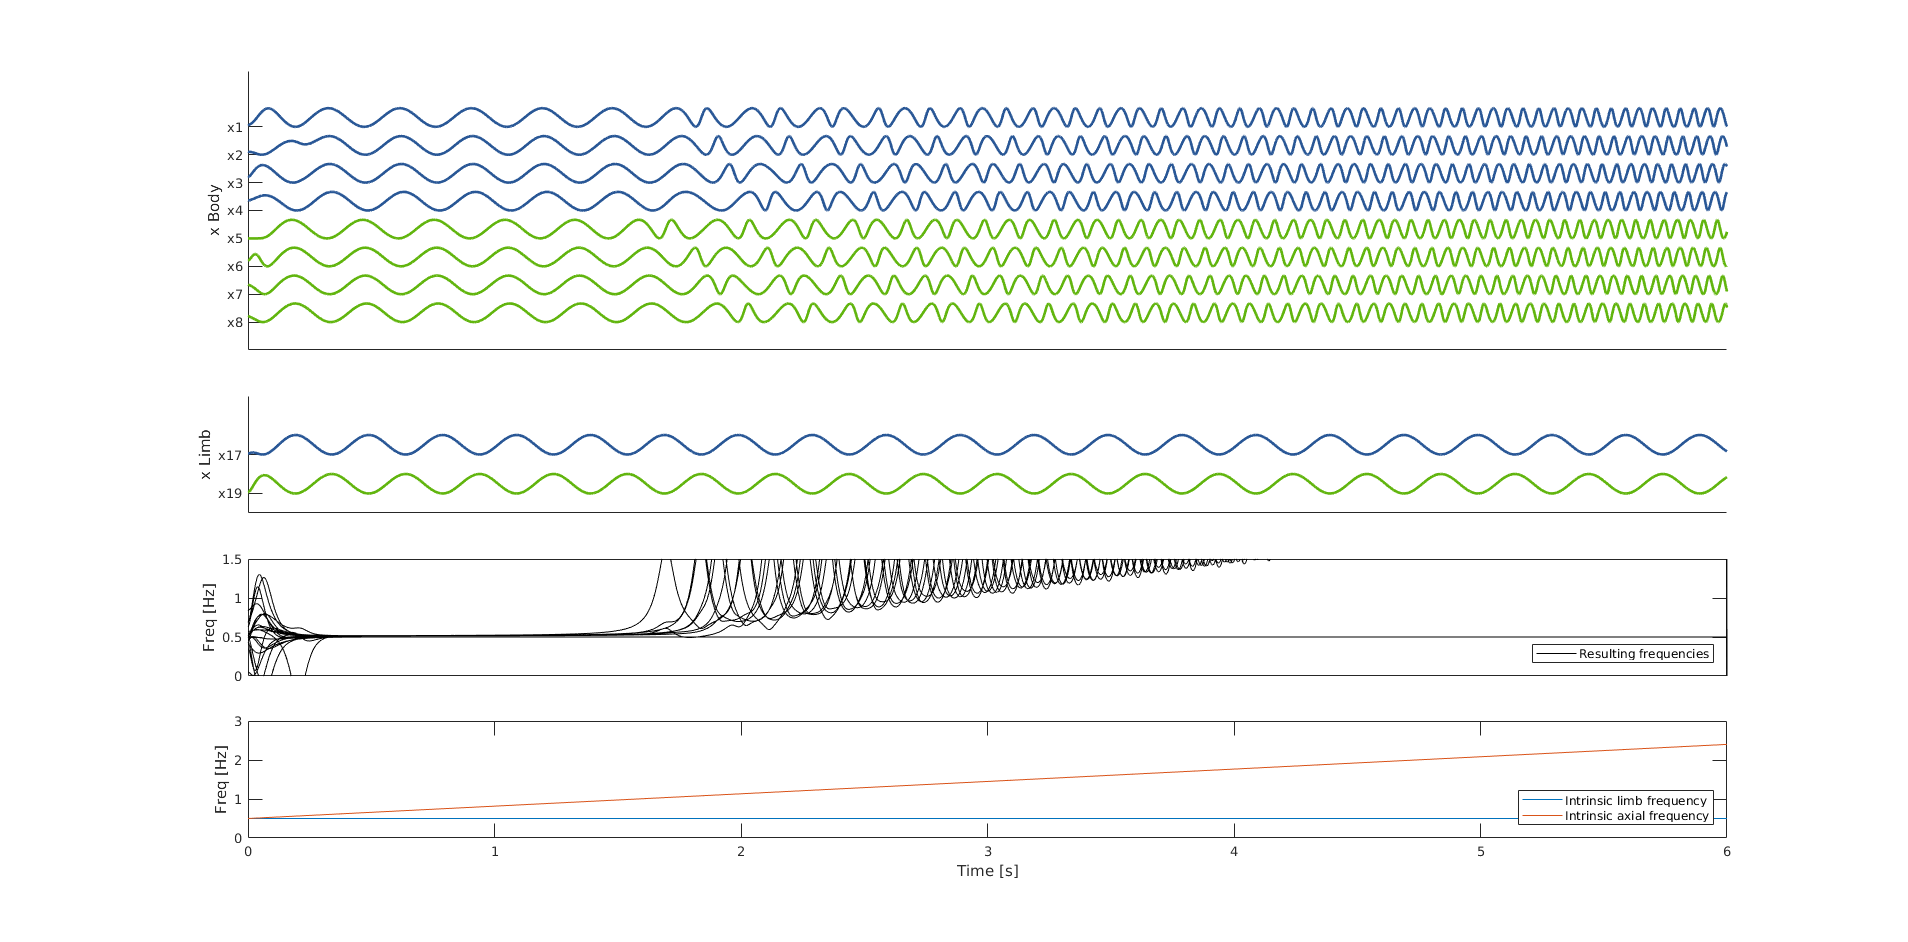
\includegraphics[width=\textwidth]{fig/figure7c_axialfreq.png}
	\caption{Simulations of the salamander CPG model applying a constant drive of 2 to achieve walking with two different values for the coupling strength between the limb oscillators (0 or 1).}
	\label{fig:7c-axialfreq}
\end{figure}

%\begin{multicols}{2}



{\setlength{\parindent}{0 cm}
of 1 they produce a messy motion between swimming and walking. However, with a strong coupling strength of 4 the limbs can finally exert a sufficient influence to force the axial oscillator to tune into a clean walking motion.
}

The limb to limb coupling was investigated in a similar way, also using a constant drive of 2 to produce walking (see figure \ref{fig:7c-limbcoupling}). This showed that the anti-phase dynamic between upper and lower limbs was lost in case of a low or non-existent limb coupling. Indeed the phase difference between the upper and lower limb was completely random and only depended on the initialization values of the system.

The next step of this section is dedicated to investigating the role of the intrinsic frequencies associated to the limb and axial oscillators. This was studied by simulating the whole system and linearly increasing the intrinsic frequency of the axial oscillators while keeping the limbs' intrinsic frequencies constant (see figure \ref{fig:7c-axialfreq}). One can observe that 2 seconds into the simulation the intrinsic frequency of the axial oscillators has already rose so much that the coupling with the limb oscillators can't contain it any more and the synchronization is lost. This is leads to a turbulent oscillation of the axial oscillators until the intrinsic axial frequency has risen to the point, at which it can seemingly decouple from the limb oscillation and the swimming dynamic starts to dominate the motion of the axial oscillators. This takeover of the intrinsic swimming motion kicks in around 4 seconds into the simulation. 

In a last step the axial contralateral coupling was also modulated. Until yet the whole analysis had \newpage only taken place on the left half of the salamander model, but the coupling between the left and right axial oscillators also plays a relevant role. If assigned to a significant value, for instance 1, this coupling strength will assure that contralateral axial oscillators should be in anti-phase. However, if it this set to zero this is no longer true as was shown by simulation using a linearly decreasing drive from 5 to 0 in order to initialize the system in swimming mode and then transit to walking (see figure \ref{fig:7c-leftright}). One can observe that in this simulation the axial oscillators have a random phase difference that depends on the initial conditions while the model is in swimming mode. However, when the drive reaches a value of 3 and the system tunes into walking mode, the intrinsic phase difference of the limbs oscillators forces contralateral limbs to be in antiphase and this dynamic is transmitted to the axial oscillators through the limb to axial oscillators coupling. This results into the contralateral axial oscillators to also assume an antipahse dynamic in synchrony with the limb oscillators.

\begin{figure*}[!b]
	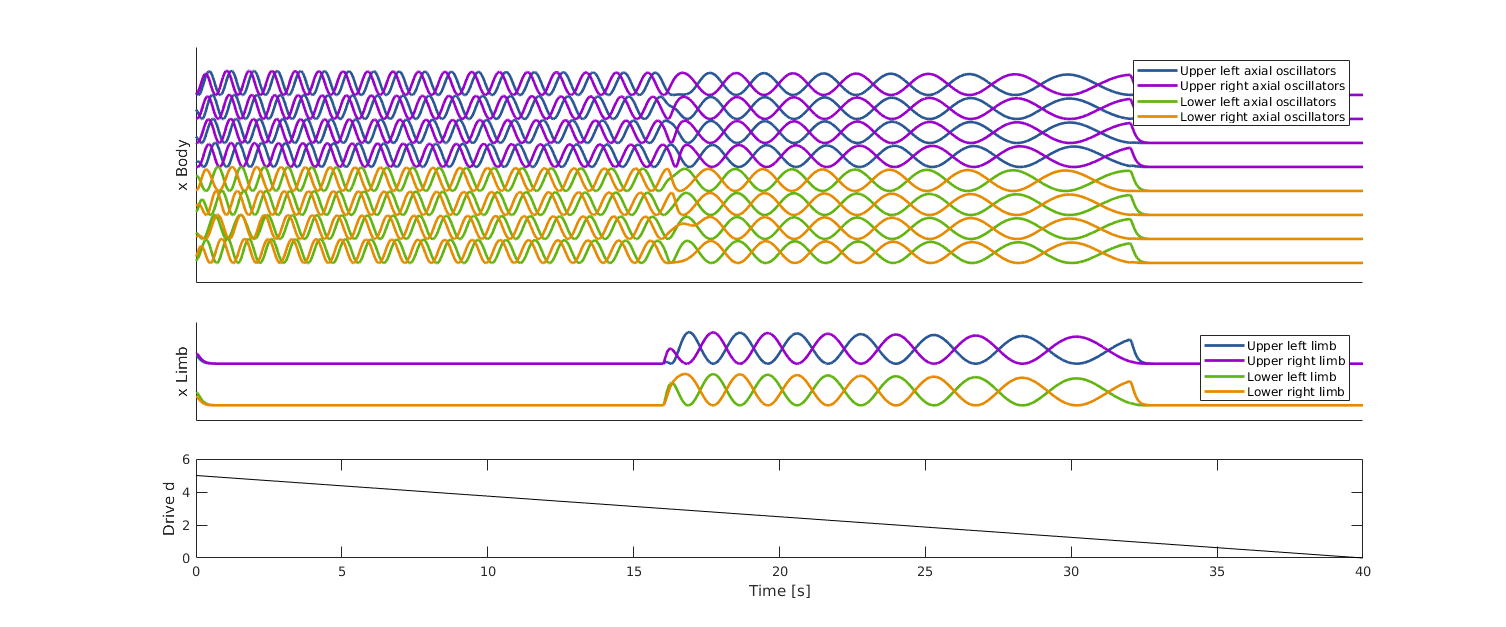
\includegraphics[width=\textwidth]{fig/figure7c_left-right-coupling.png}
	\caption{Simulation of the salamander CPG model applying a linearly decreasing drive from 5 to 0 in order to initialize the system in swimming mode and then transit into walking. The contralateral axial oscillator coupling strength is equal to zero.}
	\label{fig:7c-leftright}
\end{figure}


\section{Discussion of the model}

\section{Extensions and alternatives}

%\end{multicols}

\end{document}